\newpage

\section*{ $^{197}$Au(n,$\gamma$)$^{198}$Au }

Power Level: 100 kW(th) \\
Time at Power: 60.0 s \\
Wait Time:  2.0 h \\
Counting Time: 60.0 s \\
Total Activity at Removal: 3.50e+01 $\mu Ci$

\begin{table*}[h]
\centering
\begin{tabular}{ |c|c|c|c|c|c| }
 \hline
 Position & Mass $mg$ & Counting Activity $\mu Ci$ & Area (Counts) & Error \% \\
 \hline 
 1 & 2.91 & 7.58e+00 & 7.60e+05 & 0.1147 \\ 
\hline
 2 & 2.91 & 1.09e+01 & 1.09e+06 & 0.0957 \\ 
\hline
 3 & 2.91 & 1.02e+01 & 1.02e+06 & 0.0990 \\ 
\hline
 4 & 2.91 & 5.58e+00 & 5.59e+05 & 0.1337 \\ 
\hline
\end{tabular}
\end{table*}

\begin{figure}[h]
\centering
\begin{subfigure}{.5\textwidth}
  \centering
     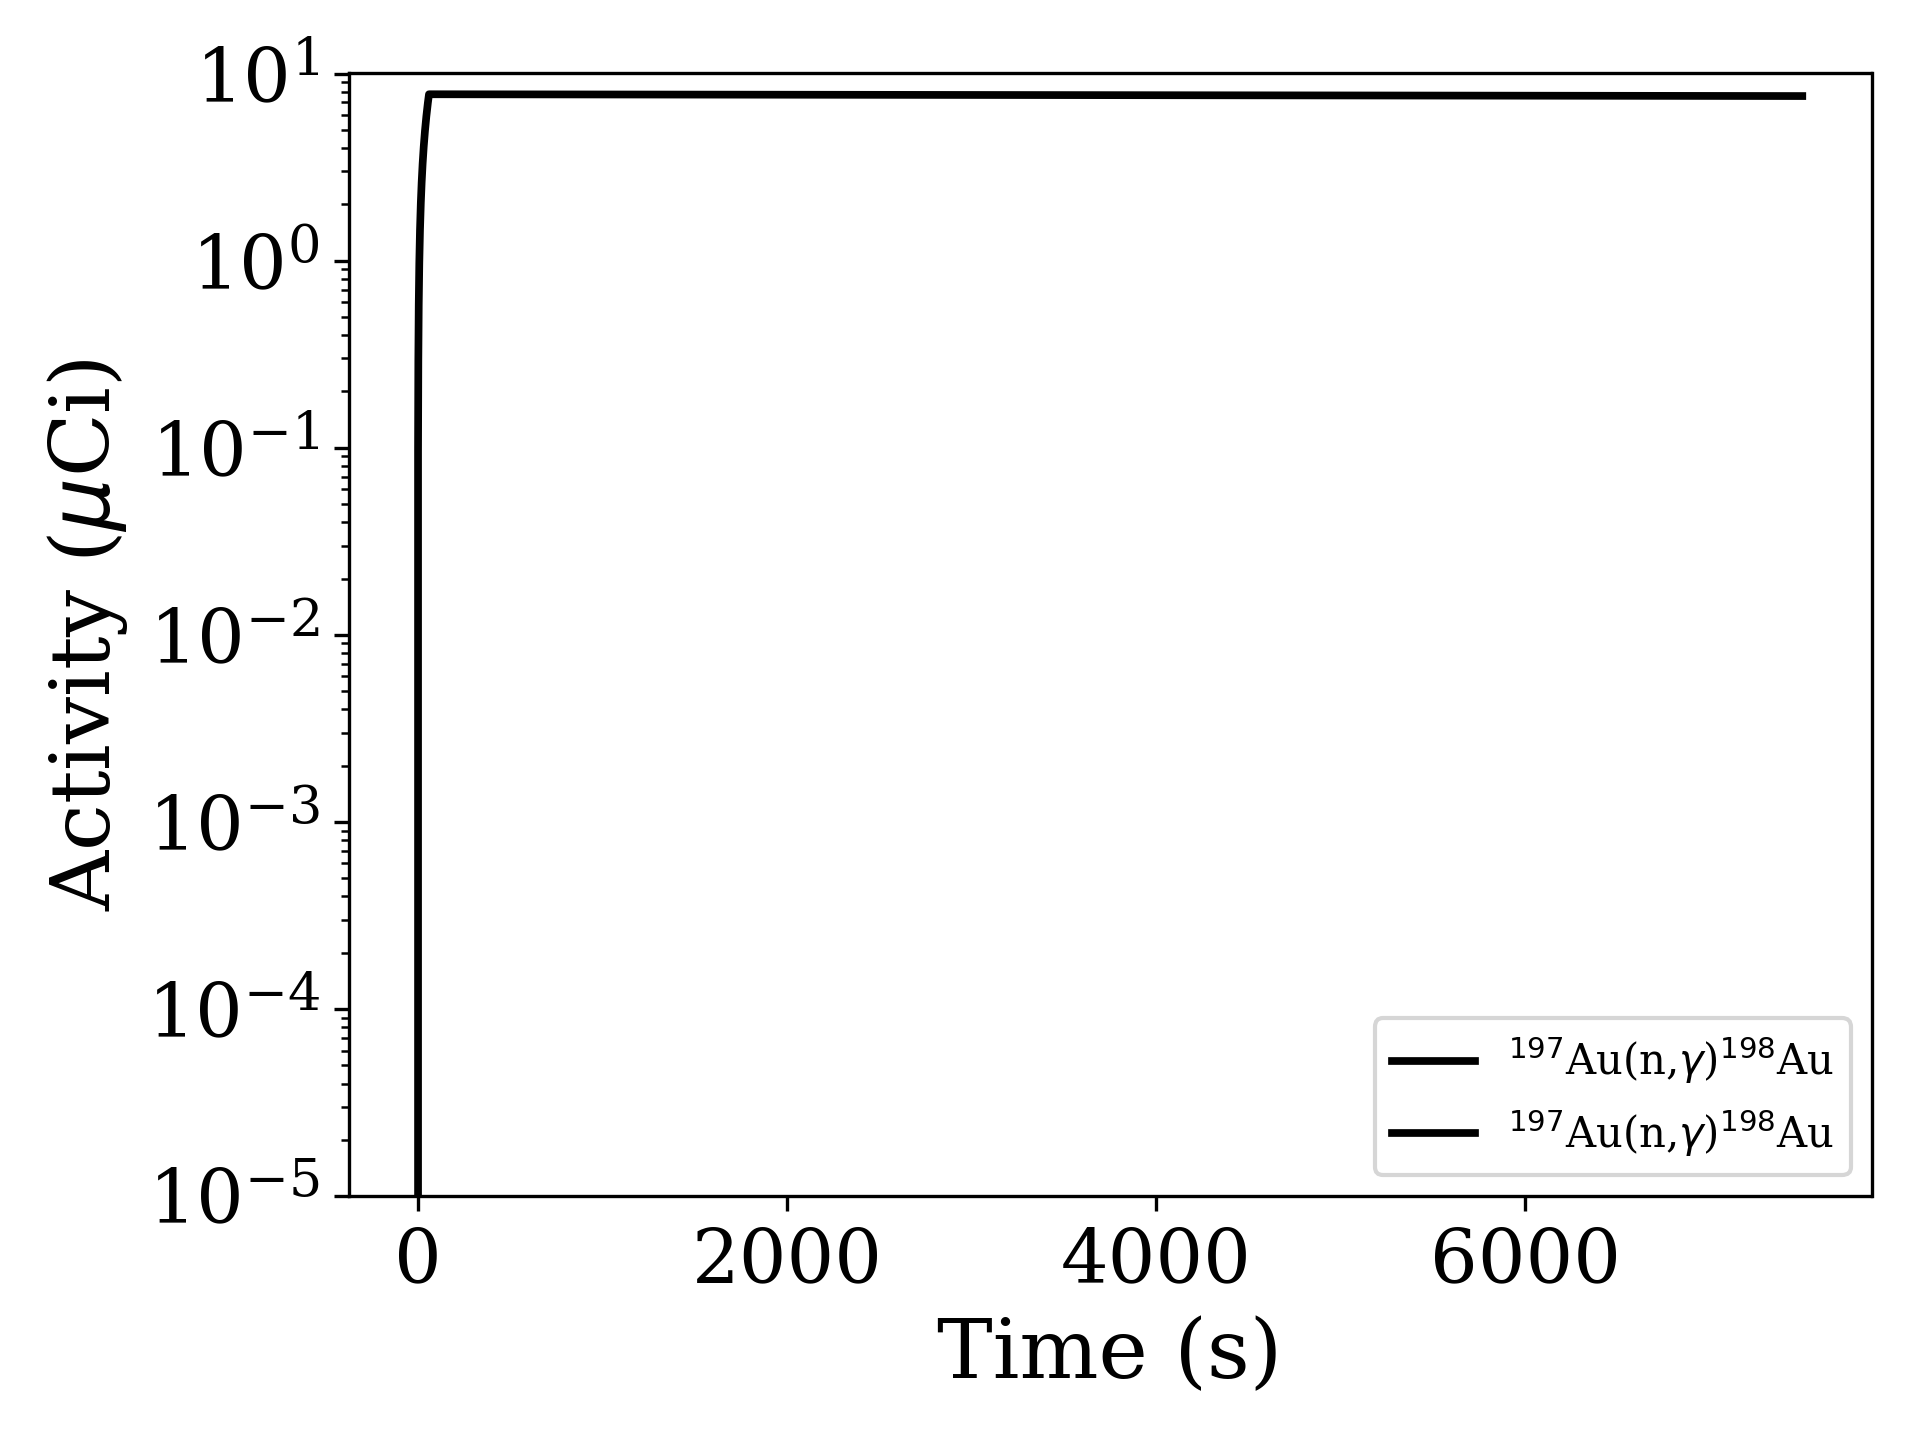
\includegraphics[width=.8\textwidth]{plot/Au-197(n,gamma)Au-198_library1} 

  \caption{A subfigure}
  \label{fig:sub1}
\end{subfigure}%
\begin{subfigure}{.5\textwidth}
  \centering
     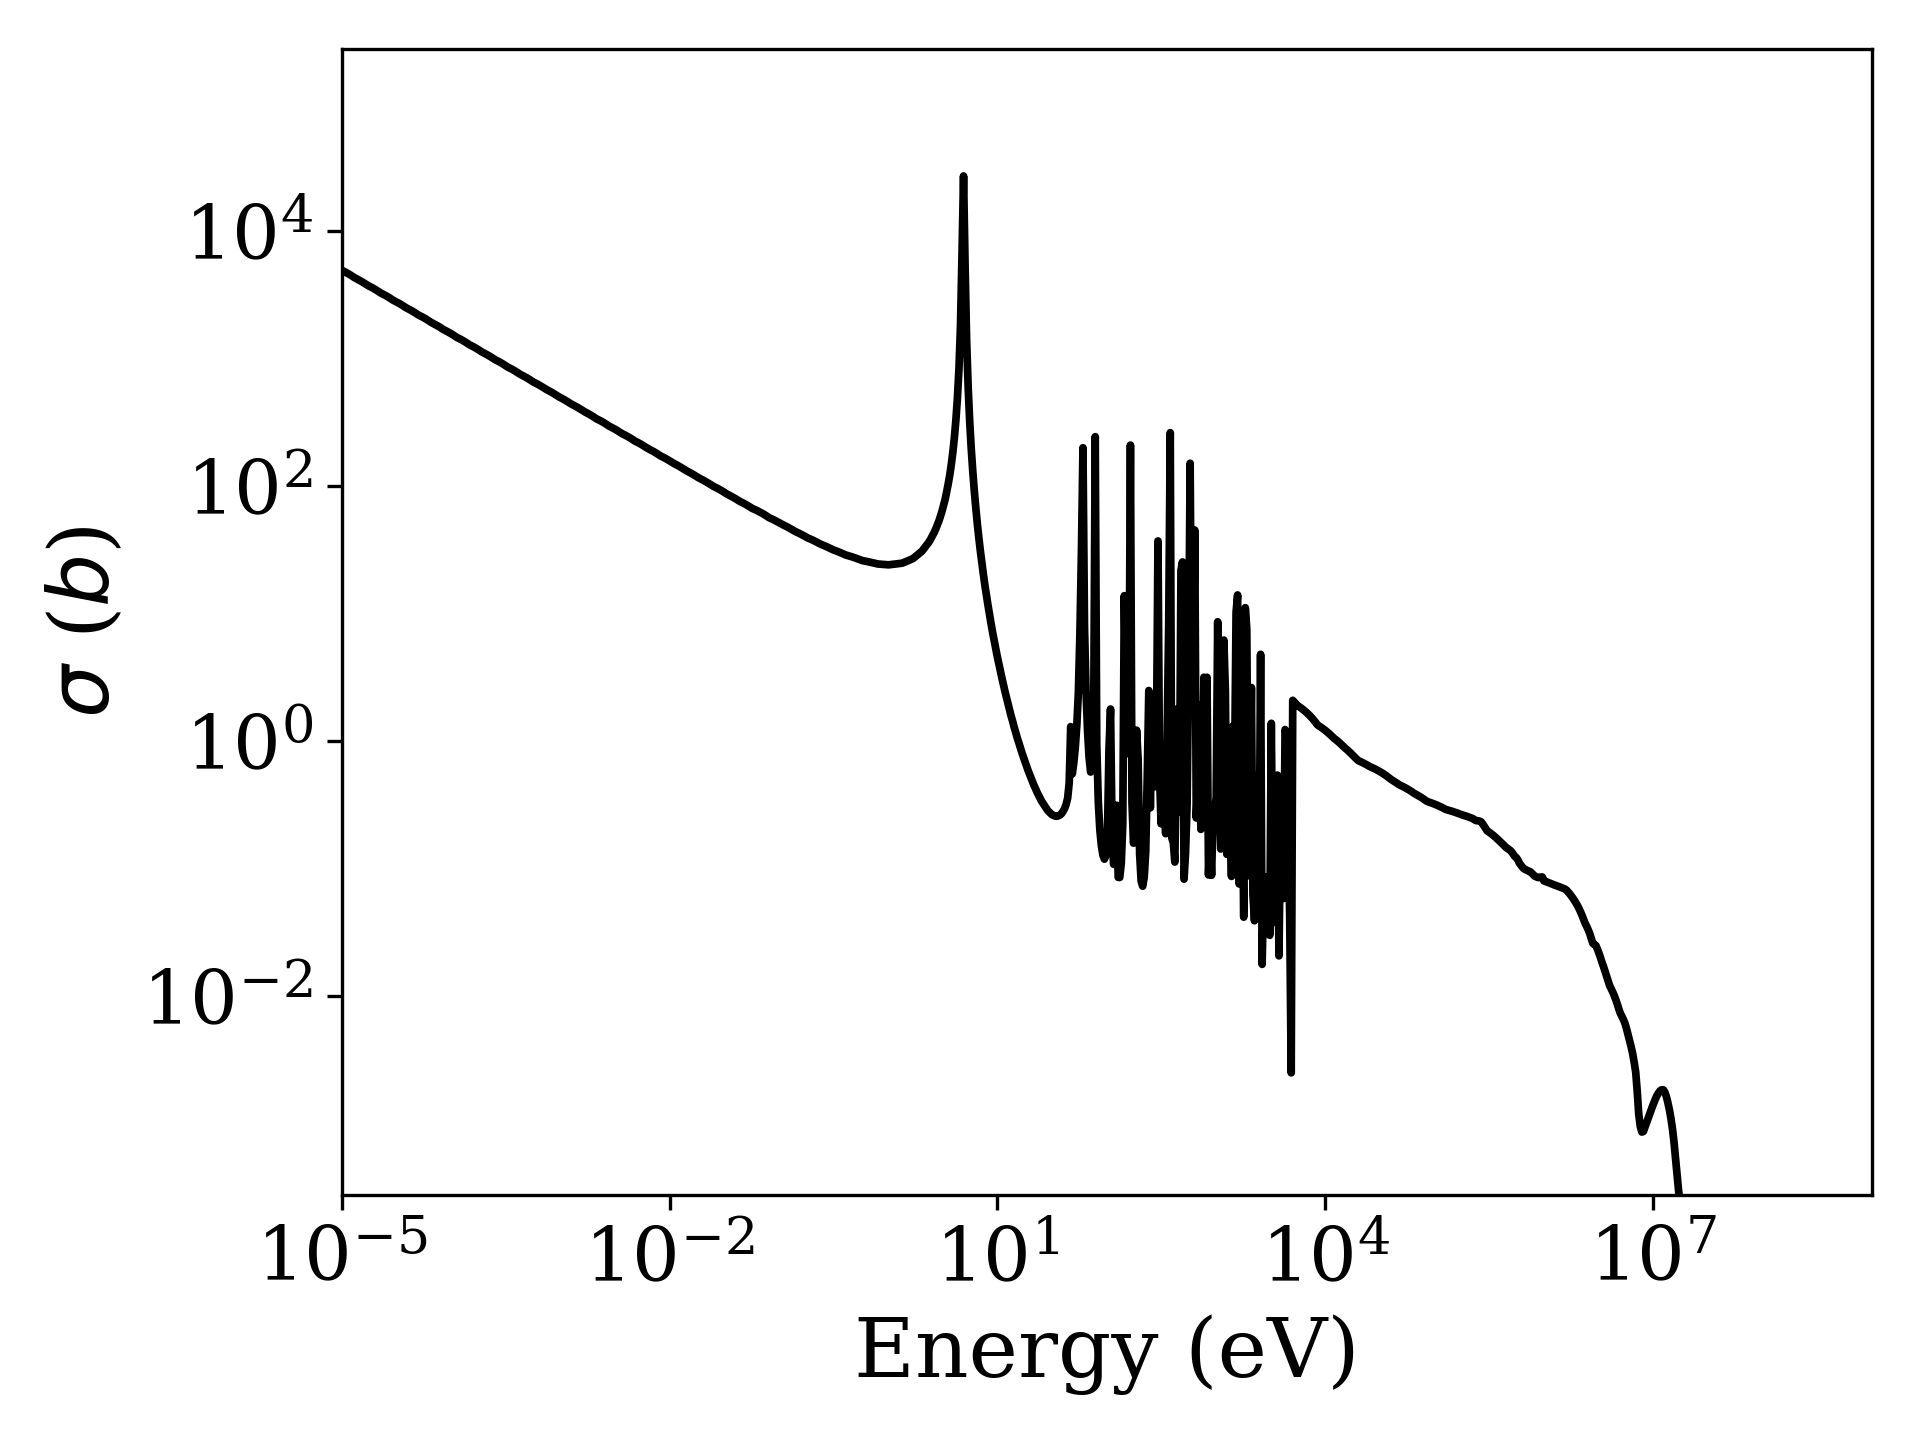
\includegraphics[width=.8\textwidth]{plot/Au-197(n,gamma)Au-198} 

  \caption{A subfigure}
  \label{fig:sub2}
\end{subfigure}
\caption{A figure with two subfigures}
\label{fig:test}
\end{figure}

\begin{table*}[h]
\centering
\begin{tabular}{ |c|c|c|c|c|c|c| }
 \hline
 Reaction & T$_{1/2}$ & ROI (eV) & Important Gammas (keV) \\
 \hline 
 $^{197}$Au(n,$\gamma$)$^{198}$Au &  2.7 d & 1.31e-02, 5.46e+00 & 412(0.95) \\ 
\hline
\end{tabular}
\end{table*}
